\subsection{28 августа. Д.р. Чиринкол}

\textit{Метеоусловия: утром, днём, вечером переменная облачность, кратковременные дожди}

\begin{figure}[h!]
	\centering
	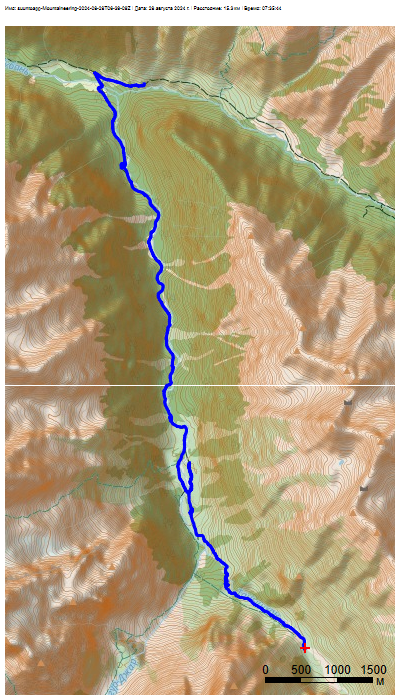
\includegraphics[angle=0, width=0.7\linewidth]{../pics/mini_maps/28}
	\label{fig:mini_28}
\end{figure}

Утром проснулись в 7:30 хорошо отдохнувшие и готовые к новому дню. В 9:40 выдвинулись вдоль левого берега реки Танышхан вниз по течению. Тропинка пролегала через россыпи курумника, заросли берез, вечнозеленых деревьев  и рододендронов - идущая впереди часть группы легко терялась из виду. Здесь мы начали встречать туристов, идущих налегке за ягодами. За 400 м до слияния с р. Чиринкол перешли на правый берег по железному мосту (N 43.27056° E 42.26168°). 
\begin{figure}[h!]
	\centering
	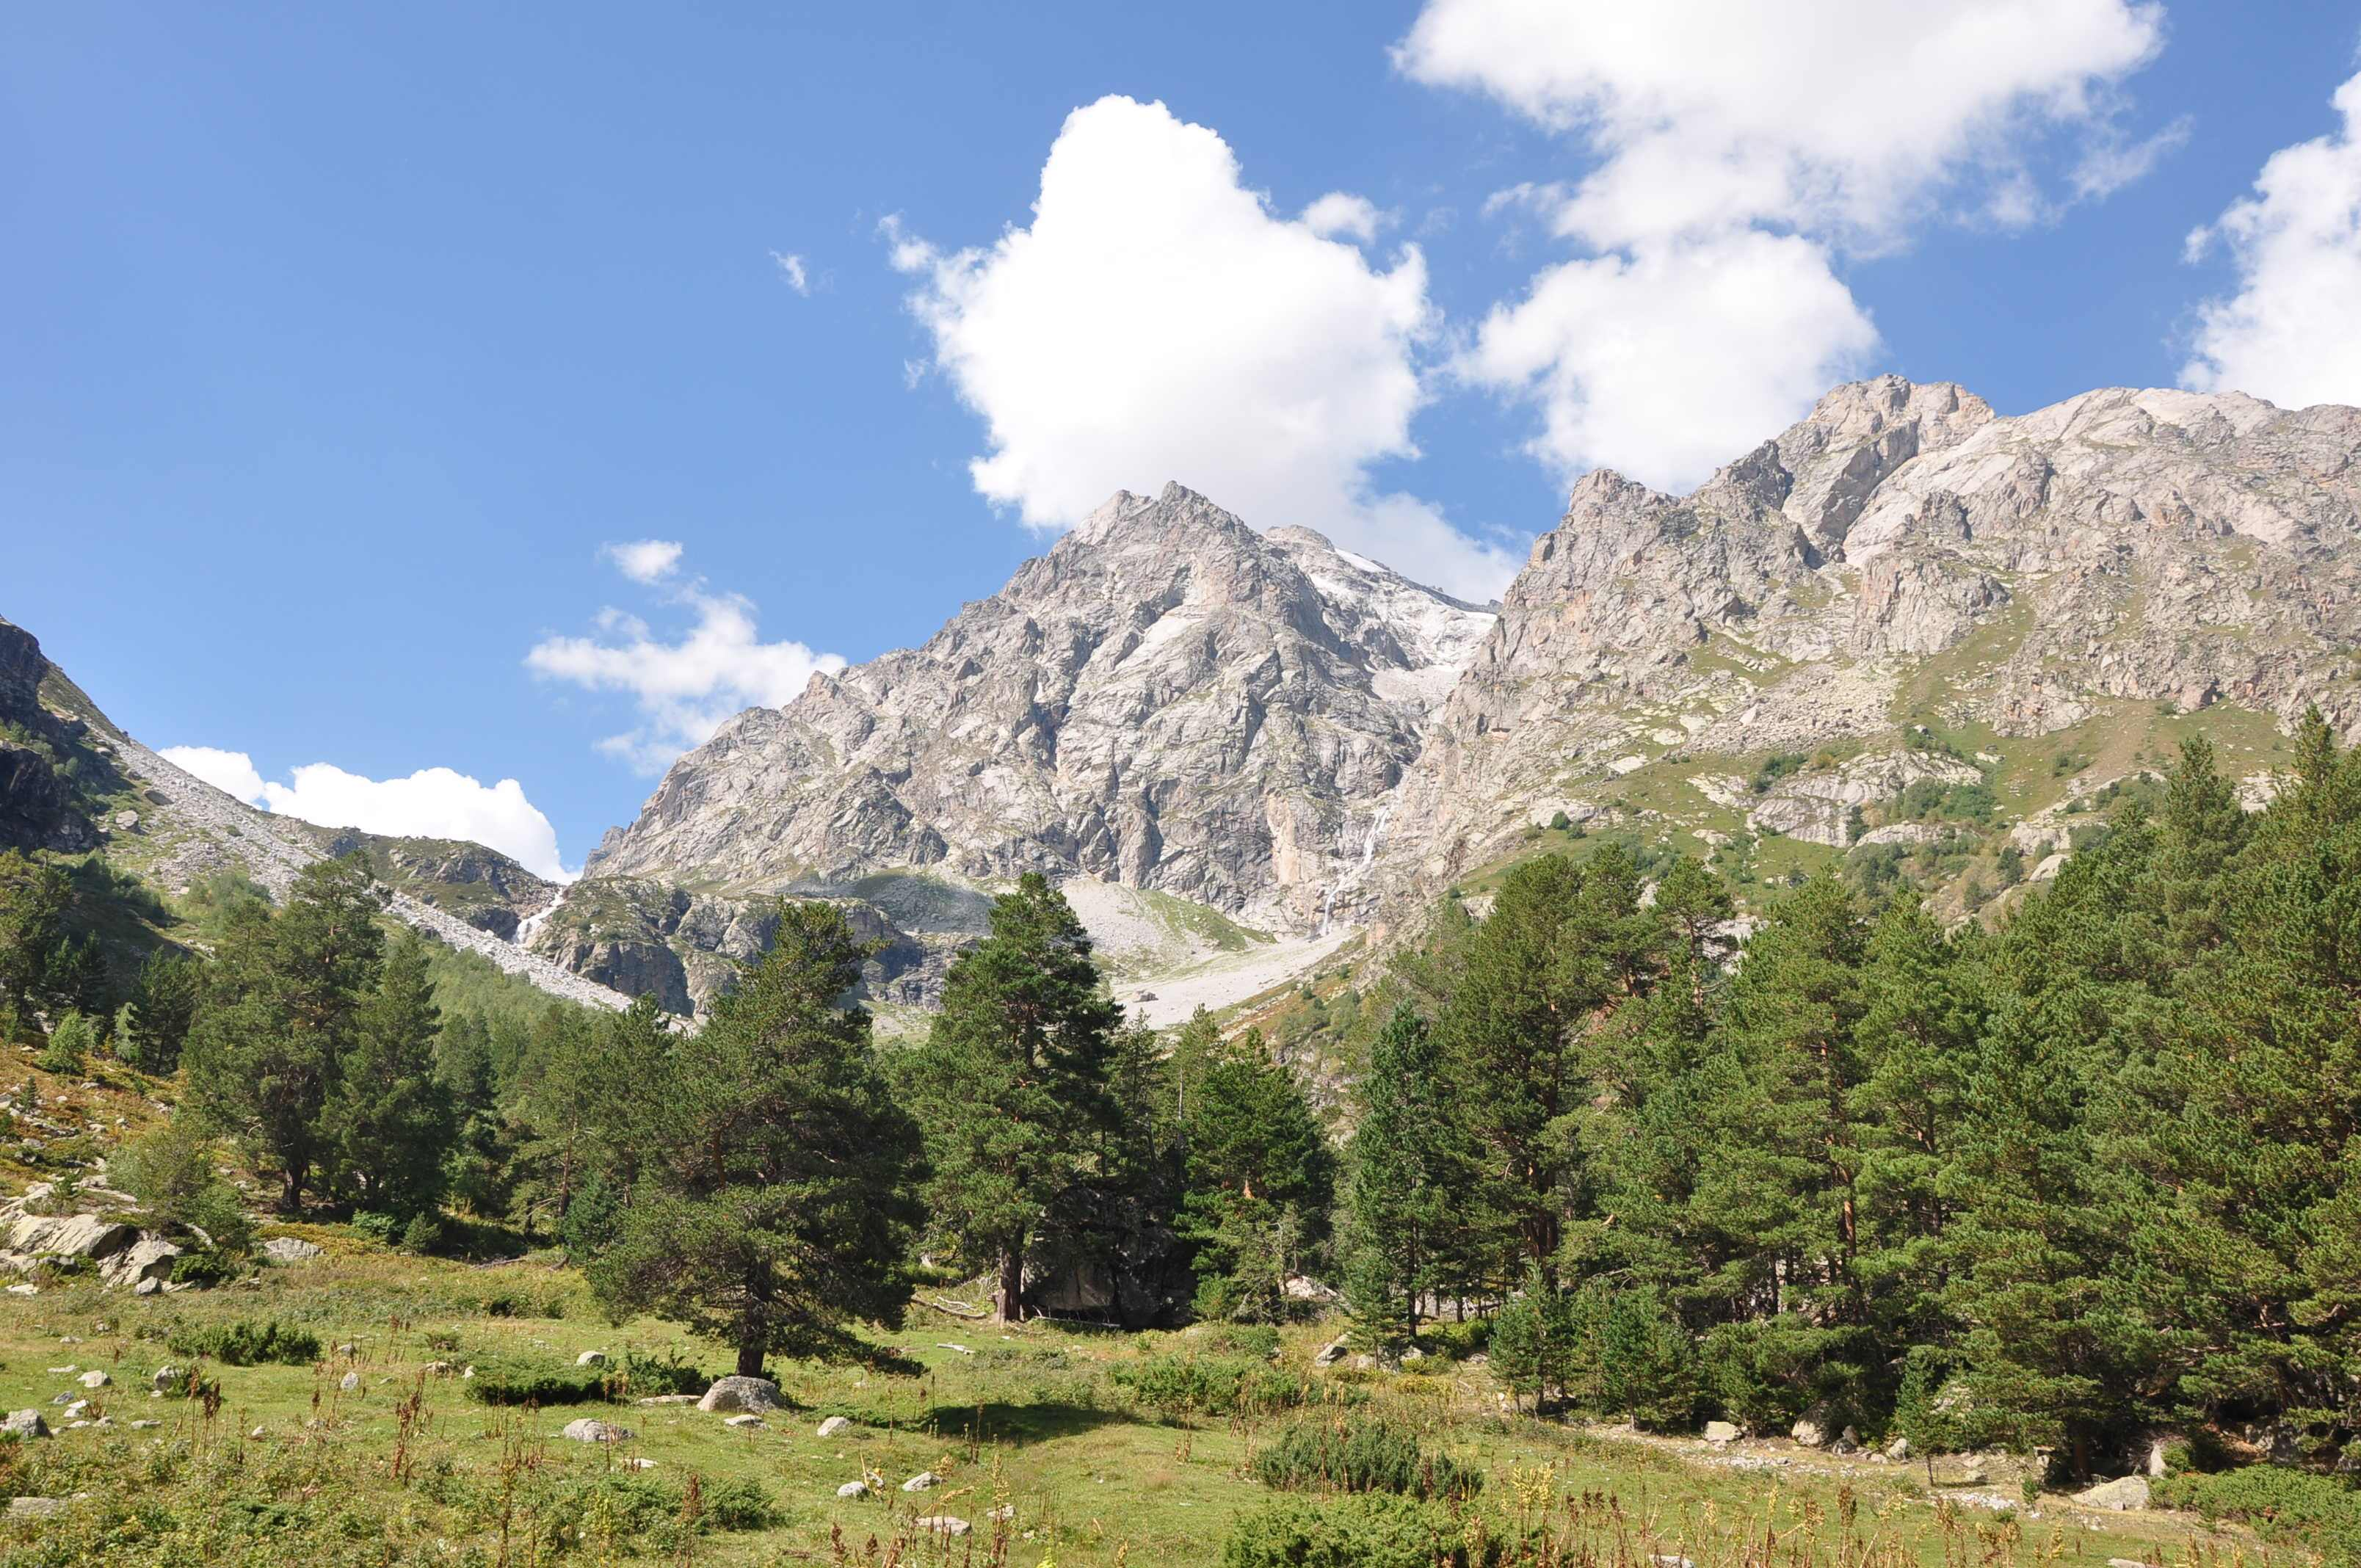
\includegraphics[width=0.7\linewidth]{../pics/DSC_0459 2}
	\caption{Берег реки Танышхан.}
	\label{fig:DSC_0459}
\end{figure}
На правом берегу в 11:10 подошли к обитаемым строениям. Повстречали как людей, так и непослушное стадо коров. Хозяйка предложила нам хычины. В 11:25 подошли к броду, но нам не повезло и уровень воды был слишком высок, чтобы не замочить ботинки. Поэтому мы вернулись назад к коровнику и перешли по бревенчатому мосту (N 43.27988° E 42.25481°).
\begin{figure}[h!]
	\centering
	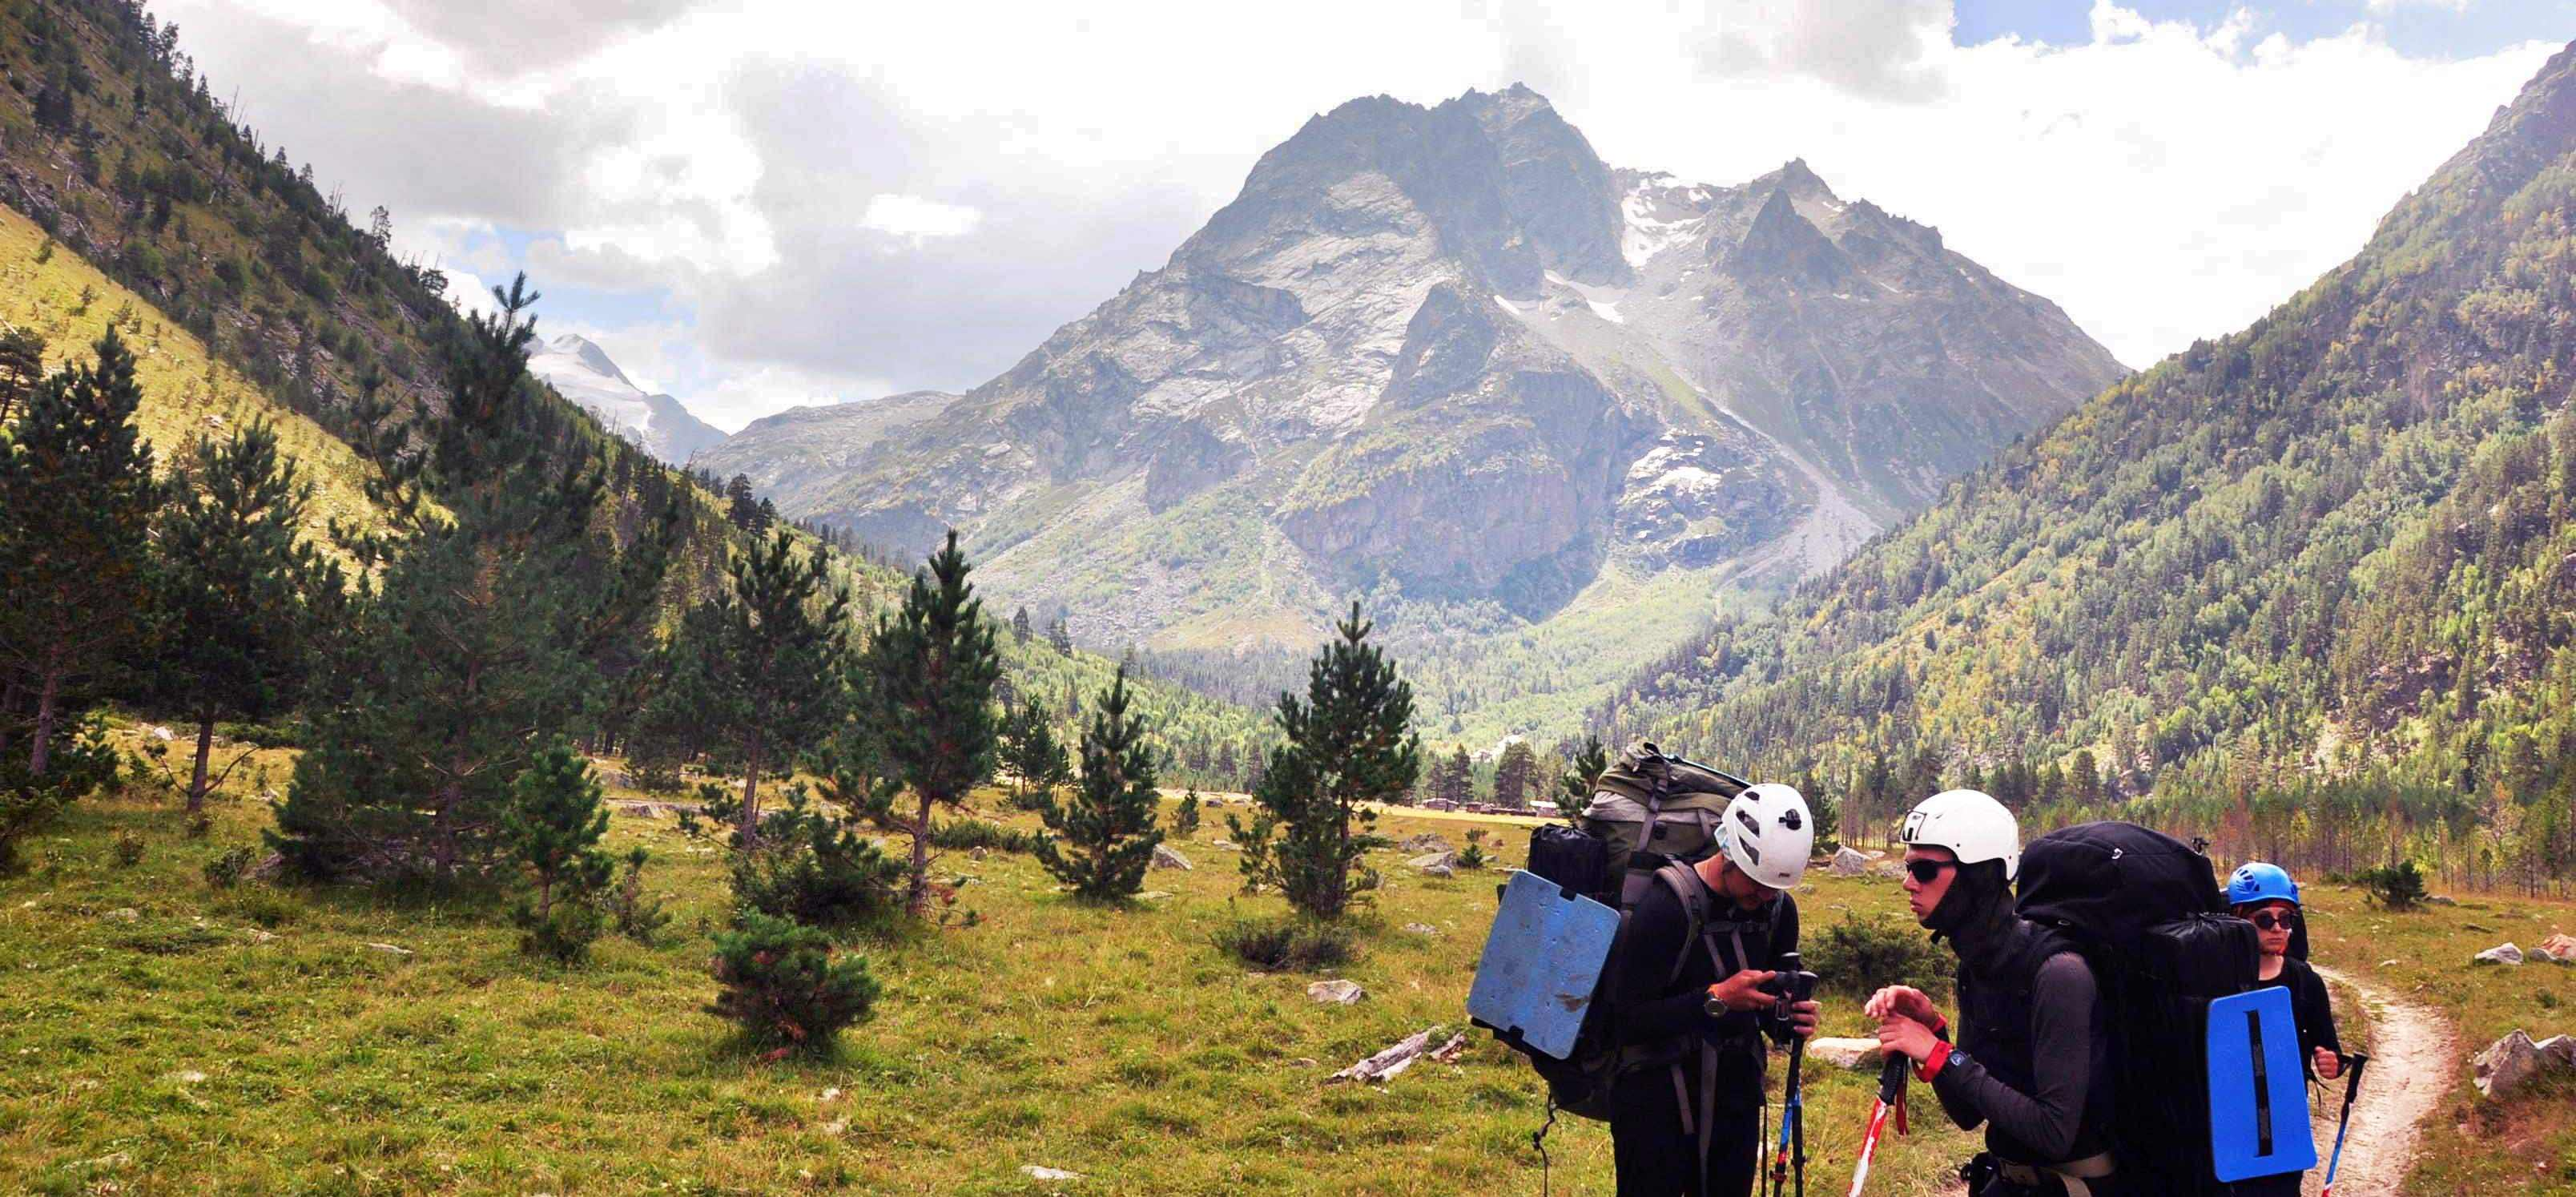
\includegraphics[width=0.7\linewidth]{../pics/DSC_0462 2}
	\caption{Рядом с бродом. На заднем плане виднеется коровник}
	\label{fig:DSC_0462}
\end{figure}

Далее шли по левому берегу р. Чиринкол по проезжей дороге. 
\begin{figure}[h!]
	\centering
	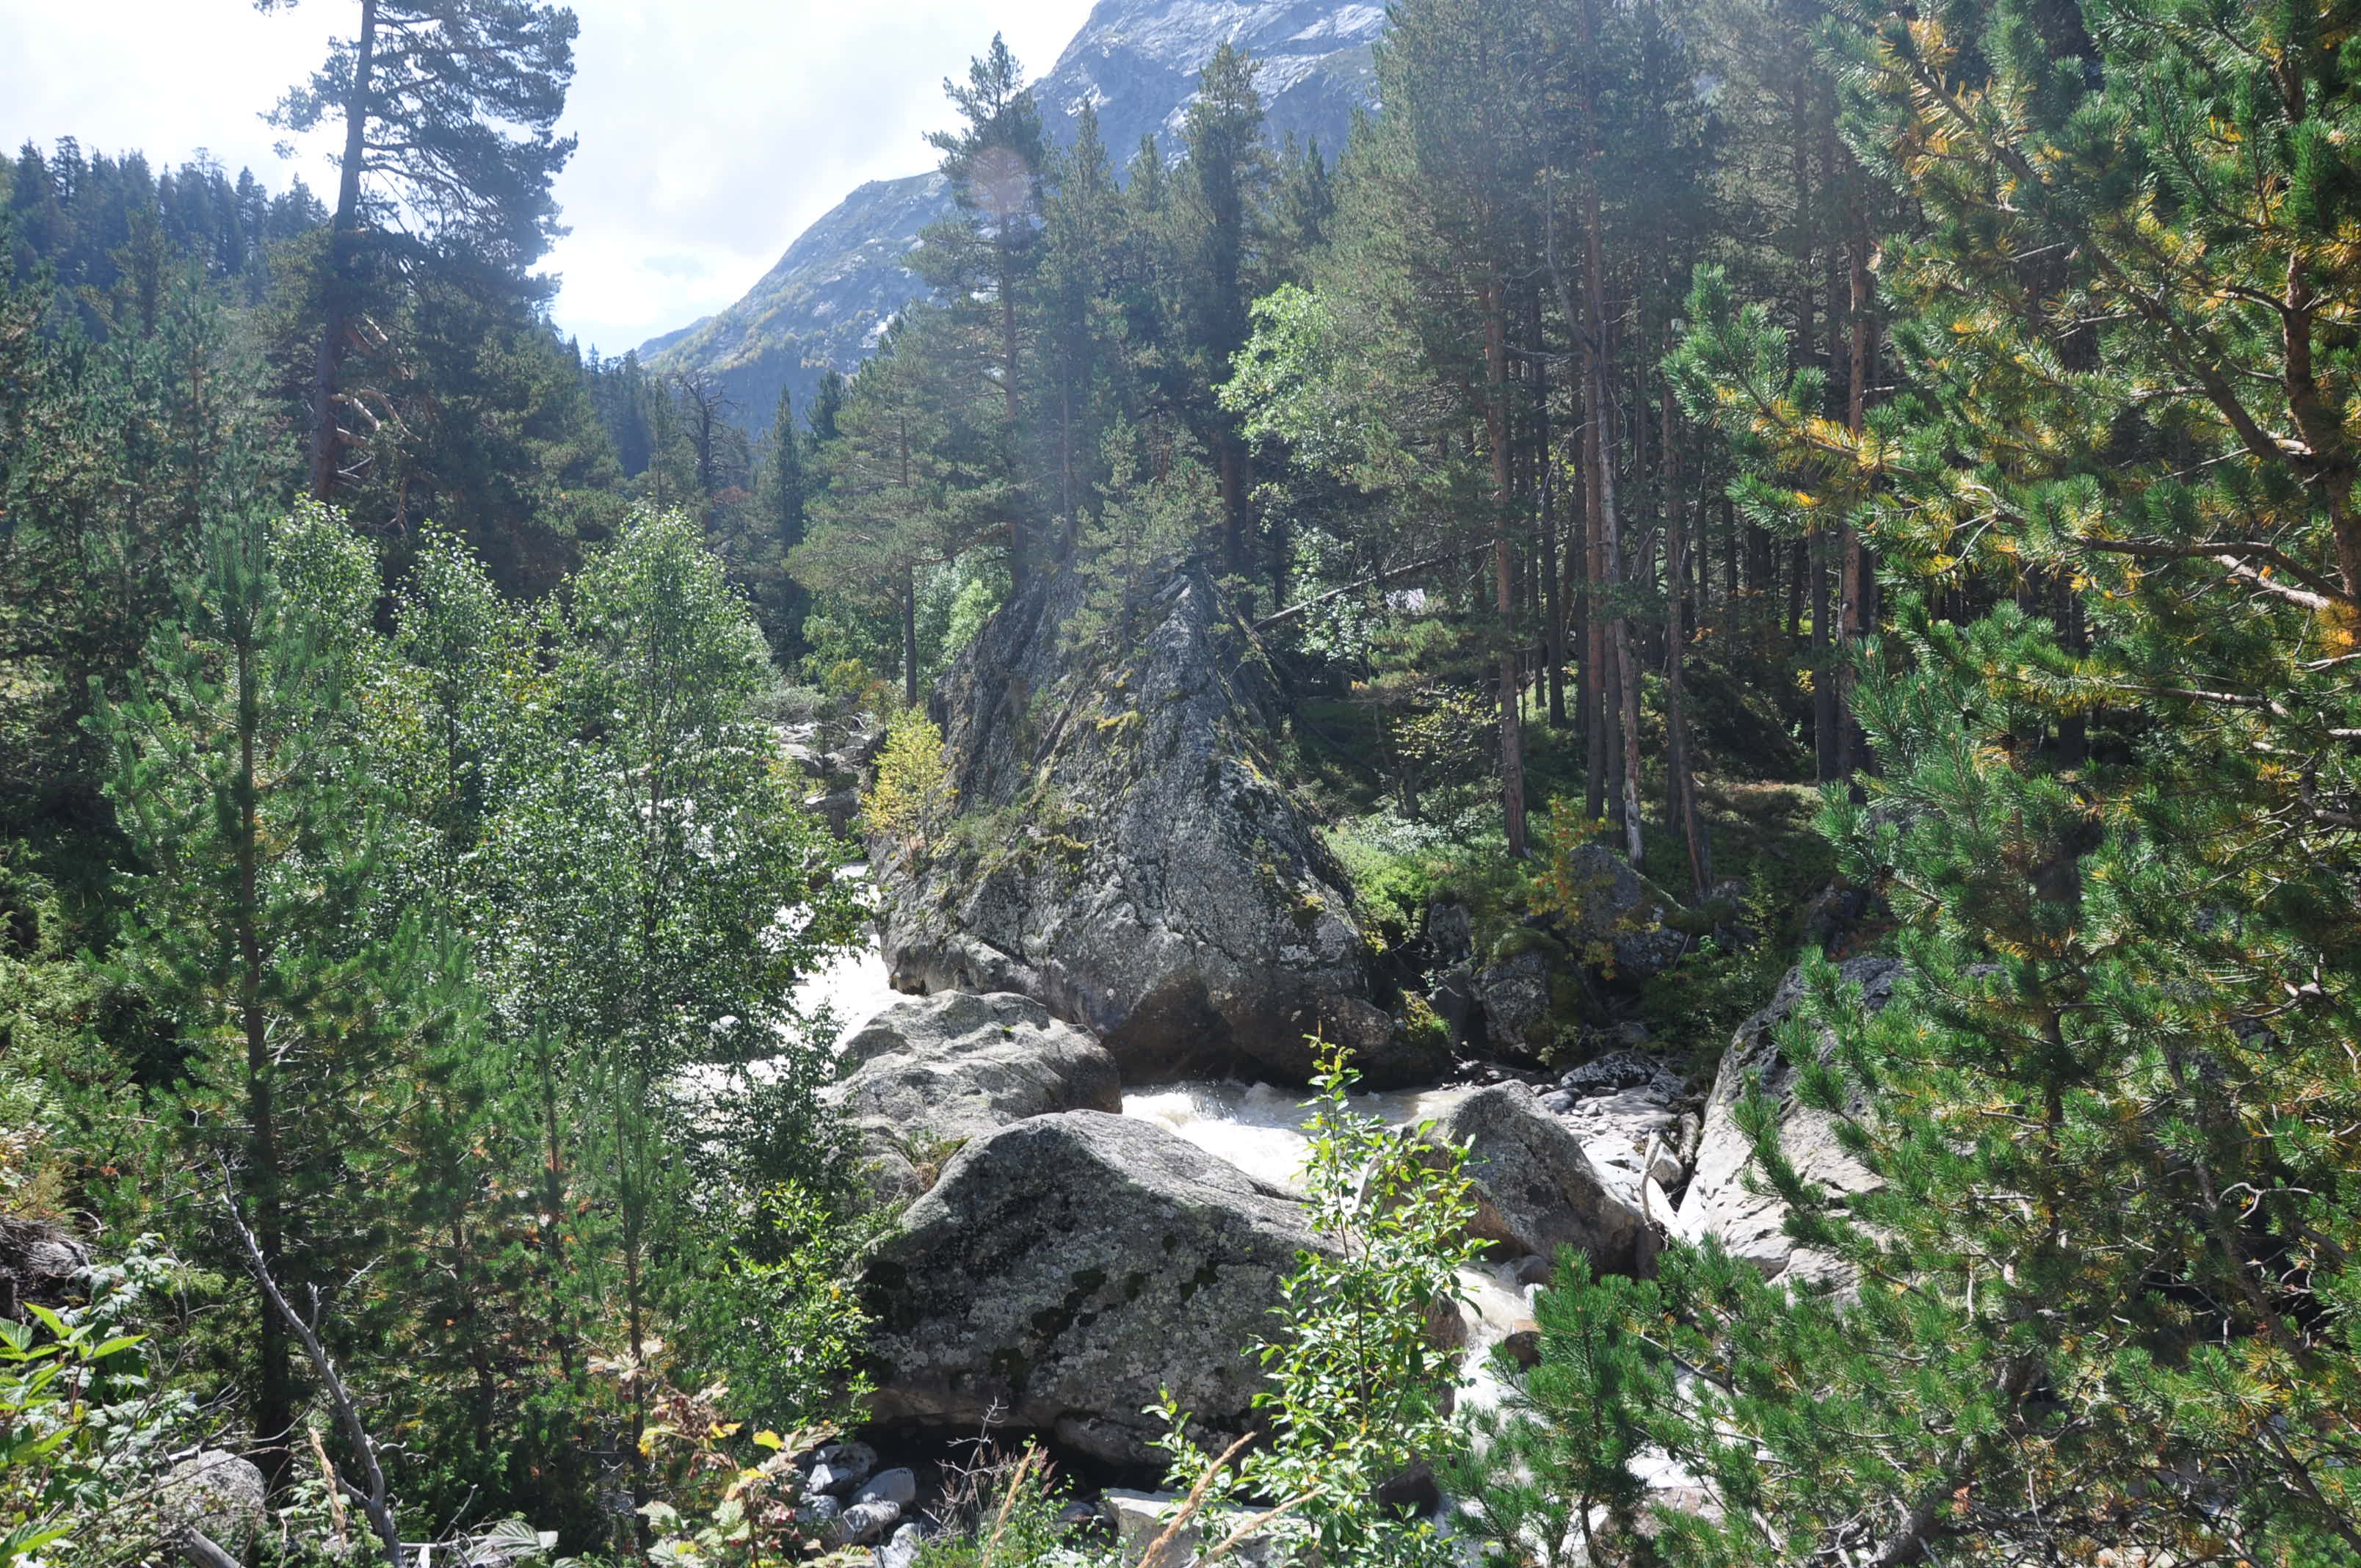
\includegraphics[width=0.7\linewidth]{../pics/DSC_0461 2}
	\caption{р. Чиринкол. Не хотелось бы в нее упасть!}
	\label{fig:DSC_0461}
\end{figure}
Пообедали в 14:14 на удобной полянке (N 43.32065° E 42.24355°). Бодро дошли до поворота на д.р. Кубань и в 17:15 встали лагерем на живописном холме (N 43.33085° E 42.24742°). Попытались поймать сеть выше по склону, но не поймали.

\clearpage